
\documentclass[tikz=true]{standalone}
\usepackage[utf8]{inputenc}

\usepackage{tikz}
\usepackage{amsfonts}
\usepackage{amsmath,amssymb}
\usepackage{systeme,mathtools}
\usetikzlibrary{positioning,arrows.meta,quotes}
\usetikzlibrary{shapes,snakes}
\usetikzlibrary{bayesnet}
\tikzset{>=latex}

\begin{document}
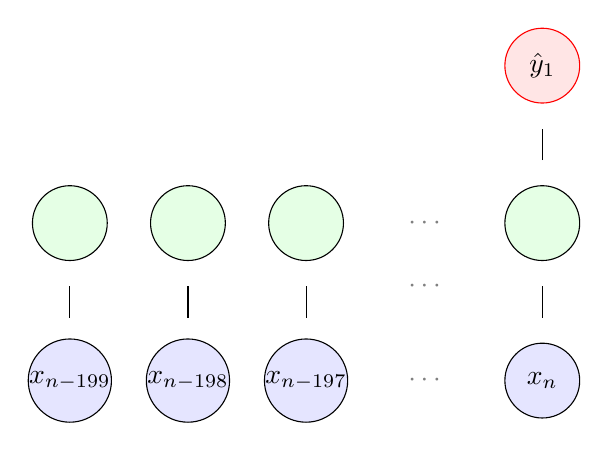
\begin{tikzpicture}

\node[circle,draw=black,fill=blue!10,inner sep=0pt,minimum size=0.95cm] (obs1) at (0,-2) {$x_{n-199}$};
\node[circle,draw=black,fill=blue!10,inner sep=0pt,minimum size=0.95cm] (obs2) at (1.5,-2) {$x_{n-198}$};
\node[circle,draw=black,fill=blue!10,inner sep=0pt,minimum size=0.95cm] (obs3) at (3,-2) {$x_{n-197}$};
\node[text width=0.4cm] (obs4) at (4.5,-2) {\color{gray}{$\cdots$}};
\node[circle,draw=black,fill=blue!10,inner sep=0pt,minimum size=0.95cm] (obsn) at (6,-2) {$x_{n}$};

\node[circle,draw=black,fill=green!10,inner sep=0pt,minimum size=0.95cm] (rnn1) at (0,0) {};
\node[circle,draw=black,fill=green!10,inner sep=0pt,minimum size=0.95cm] (rnn2) at (1.5,0) {};
\node[circle,draw=black,fill=green!10,inner sep=0pt,minimum size=0.95cm] (rnn3) at (3,0) {};
\node[text width=0.4cm] (obs4) at (4.5,0) {\color{gray}{$\cdots$}};
\node[circle,draw=black,fill=green!10,inner sep=0pt,minimum size=0.95cm] (rnnn) at (6,0) {};

\draw[] (0,-0.8) -- (0,-1.2);
\draw[] (1.5,-0.8) -- (1.5,-1.2);
\draw[] (3,-0.8) -- (3,-1.2);
\node[text width=0.4cm] (obs4) at (4.5,-0.8) {\color{gray}{$\cdots$}};
\draw[] (6,-0.8) -- (6,-1.2);


\node[circle,draw=red,fill=red!10,inner sep=0pt,minimum size=0.95cm] (out1) at (6,2) {$\hat{y}_{1}$};
\draw[] (6,0.8) -- (6,1.2);

\end{tikzpicture}
\end{document}
